\chapter{Simulation Structure}\label{simulation_structure}

%%%%%%%%
%%%%%%%% Simulation Environment
%%%%%%%%
\section{Simulation Environment}\label{simulation_environment}
Goes over the backend design

%%%%%%%%
%%%%%%%% Simulation Flow
%%%%%%%%
\section{Simulation Flow}\label{simulation_flow}
The order in which events happen
Need a nice diagram for this

%%%%%%%%
%%%%%%%% Message Passing
%%%%%%%%
\section{Message Passing}\label{message_passing}
\subsection{Primitive Messaging}
An important role of Team 1 was to design a mechanism for agents to talk amongst each other in the simulation that would allow automated communication. The first step in this process was to design a system which would allow an agent to pass along a minimum viable message to their neighbours. These were the goals of communication in the MVP:
\begin{itemize}
    \item Agents could only talk to their immediate neighbors (+/- 1 floor).
    \item Agents should be given the ability to ignore communication.
    \item Multiple agents could be “speaking” at a given tick.
    \item One agent could send one message per tick.
    \item \textbf{It is entirely an agent's discretion if/when/how they wish to react to a message as long as their behavior is not deceptive}
\end{itemize}
As a team, Team 1 emphasized the last point. The infrastructure should not force any behavior onto the agent as long as the behavior was honest. The basic philosophy of the communication infrastructure was to dictate as little as possible about the agent's behavior while keeping the API friendly, readable and hard to get wrong. This usually meant making providing basic override-able behaviors to be as unobtrusive as possible to team strategies. \newline
The minimum default message had to have the following fields that are accessible to all the agents that receive it:
\begin{itemize}
    \item \textbf{\texttt{MessageType}}: Indicates one of 13 enumerated message types.
    \item \textbf{\texttt{SenderFloor}}: Returns the floor this message was sent from.
    \item \textbf{\texttt{TargetFloor}}: The floor the message is addressed to.
    \item \textbf{\texttt{ID}}: Each message sent is given a unique ID.
\end{itemize}
\vspace{\baselineskip}
For the MVP, Team 1 constructed a system where for example in a scenario where Alice (currently at floor 10) wishes to send a message upward:
\begin{enumerate}
    \item At Tick 0, Alice would construct the message for Bob containing the following information:
        \begin{itemize}
            \item \textbf{Alice's ID}
            \item \textbf{Alice's current floor}: 30
            \item \textbf{Message's target floor}: 31 \textit{Since Alice wants to message the floor above her}
            \item \textbf{Message Type} (to be elaborated on the Common Languages Section)
        \end{itemize}
    \item Still at Tick 0, Alice calls \texttt{SendMessage} which takes her message and passes it to the tower.
    \item The tower acts as the communication authority, finding the agent who is on floor 31 at Tick 0 and inserts the message into the recipient agent's (Bob's) inbox.
    \item At Tick 1, Bob may choose to call \texttt{ReceiveMessage} which would extract Alice's message (if Alice was the first or only agent to send him a message at Tick 0) and respond.
    \item If Bob has called \texttt{ReceiveMessage}, Alice's message is removed from Bob's inbox.
\end{enumerate}
With this implementation, each agent is responsible for calling \texttt{ReceiveMessage} once per tick to receive any messages. The inbox is FIFO - If multiple messages were received or if there were outstanding messages from previous ticks, only the earliest one can be retrieved at a given tick.

Additionally, "receiving" does not necessarily imply "reacting", an agent is capable of receiving a message and not responding to it at all without the sender's knowledge. Decoupling "receiving" and "reacting" gave agent teams the freedom to ignore messages entirely (metaphorically covering their ears in the tower and refusing to listen to anybody), to listen to messages and do nothing about them, or to actively listen and react. \newline
Beyond the MVP, however, messages needed to have meaning. Because the process would be automated it was meaningless to send unstructured strings, how was an agent to understand ``Please only eat what you need to survive."? \newline
A common language was necessary.

\subsection{Common Language}
To design the common language, Team 1 surveyed the agent teams asking for what they would like to talk to other agents about. We collected suggestions and found that communication indicated one of four possibilities:
\begin{enumerate}
    \item An agent could be \textit{asking} another agent for information. ``How much food is on the platform when it gets to you?" or ``How much food did you take?"
    \item An agent could be \textit{stating} something about its state or environment. ``I am in critical (health) condition" or ``There is no more food left on the platform"
    \item An agent could be \textit{request} something from another agent. ``Please leave 10 food on the platform for me."
    \item An agent could be \textit{responding} to another agent's request. ``Yes." or ``No."
\end{enumerate}
These categories solidified into four basic messages - \texttt{Ask}, \texttt{State}, \texttt{Request}, and \texttt{Response}. \newline
In addition, \texttt{Ask} and \texttt{Request} are messages that expect a response. A \texttt{State} message could be a response to an \texttt{Ask} but also could be an unprompted announcement while \texttt{Response} must be responding to some pre-existing \texttt{Request}. \newline 
While Team 1 did not want to force agent teams into any behaviors, we wanted to make the API compatible with the expected etiquette of communication. This lead to the message categorization and pair-wise reply functionality summarized below.
\begin{center}
\begin{tabular}{p{3cm}p{3cm}p{5cm}p{3.5cm}}
 \hline
 \textbf{Message \newline Category} & \textbf{Reply \newline Category} & \textbf{Body Functions} & \textbf{Description} \\ [0.5ex] 
 \hline\hline
 \texttt{AskMessage} & \texttt{StateMessage} &  \texttt{Reply}: Returns appropriate statement & Inquires something about a neighboring agent's state. \\
 \hline
 \texttt{StateMessage} & N/A & \texttt{Statement}: Returns the value of statement. \textit{e.g. a StateHP message of 5HP would return 5.} & Announces something about an agent's state or environment. \\ 
 \hline
 \texttt{RequestMessage} & \texttt{ResponseMessage} & \texttt{Reply}: Returns \texttt{BoolResponse} \newline \texttt{Request}: Returns the value of a request \textit{e.g. a RequestLeaveFood message that requests an agent to leave 10 food would return 10 on \texttt{Request}} & Asks how much food is on the platform when it arrives at the (recipient) agent \\ 
 \hline
 \texttt{ResponseMessage} & N/A & N/A & Asks how much food an agent is planning to take \\ 
 \hline
\end{tabular}
\end{center}
From these basic categories 11 specific messages were developed that specified what was being asked, stated, requested or responded to.
\begin{center}
\begin{longtable}{p{4cm}p{2.5cm}p{4cm}p{4cm}}
 \hline
 \textbf{Message Type} & \textbf{Category} & \textbf{Description} & \textbf{Reply Type} \\ [0.5ex] 
 \hline\hline
 \texttt{AskFoodTaken} & \texttt{AskMessage} & Asks how much food an agent has (already) taken
 & \texttt{StateFoodTaken} \\ 
 \hline
 \texttt{AskHP} & \texttt{AskMessage} & Asks how much HP an agent has & \texttt{StateHP} \\ 
  \hline
 \texttt{AskFoodOnPlatform} & \texttt{AskMessage} & Asks how much food is on the platform when it arrives at the (recipient) agent & \texttt{StateFoodOnPlatform} \\ 
 \hline
 \texttt{AskIntendedFoodIntake} & \texttt{AskMessage} & Asks how much food an agent is planning to take & \texttt{StateIntendedFoodIntake} \\ 
 \hline
 \texttt{StateFoodTaken} & \texttt{StateMessage} & States how much food an agent has taken &   \\
 \hline
 \texttt{StateHP} & \texttt{StateMessage} & States how much HP an agent has &   \\
 \hline
 \texttt{StateFoodOnPlatform} & \texttt{StateMessage} & States how food is on the platform when it arrives to the agent &  
 \\
 \hline
 \texttt{StateIntendedFoodIntake} & \texttt{StateMessage} & States how food the agent is planning to take &  
 \\
 \hline
 \texttt{RequestLeaveFood} & \texttt{RequestMessage} & Requests that an agent (presumably above) you leaves a certain amount of food on the platform & \texttt{BoolResponse}
 \\
 \hline
 \texttt{RequestTakeFood} & \texttt{RequestMessage} & Requests that an agent (presumably above) you takes a certain amount of food on the platform & \texttt{BoolResponse}
 \\
 \hline
 \texttt{BoolResponse} & \texttt{ResponseMessage} & Message affirming or rejecting a request &  
\end{longtable}
\end{center}
The distinction between "receiving" and "reacting" becomes important. Because we wanted to ensure that \textit{receiving} any of these message types did not mean that the recipient had to \textit{react}, the "reaction" was separated into an external function which the agent could optionally call after they extracted their message from the inbox. \newline
The design works such that if Alice on Floor 11 wanted to ask Floor 12 to leave 10 food on the platform for her:
\begin{enumerate}
    \item At Tick 0, Alice constructs a \texttt{RequestLeaveFoodMessage} with \texttt{Request} set to 10 addressed to Floor 12.
    \item At Tick 0, Alice sends the message.
    \item At Tick 1, Bob (whose inbox was previously empty and who was listening for messages) receives Alice's message. If he chooses to react, he decides whether or not he wants to cooperate with Alice and generates his response with the \texttt{Reply} function of the message (no need to construct the \textit{BoolResponseMessage} himself).
    \item At Tick 1, he sends his reply back, addressed to the message's sender floor.
    \item At Tick 2, Alice (whose inbox was also previously empty) receives Bob's response and may choose to react to it.
\end{enumerate}
The system so far provided a solid mechanism for agents to communicate to their neighbours, to gather information and to request help in times of crisis (potentially building trust or temporary relationships). However, it was contingent on communicating agents being on consecutive floors, any relationships built through this kind of communication could only last for a reshuffle period unless the agent implemented a specific kind of internal memory structure. Additionally, the communication was still relatively rudimentary. Alice's request for 10 food could be rejected by Bob because his HP is critical and he will starve immediately without food, but the current system only allows Bob to either accept or refuse Alice's request without communicating anything about his own state. This could potentially worsen his relationship with Alice, had Alice known that Bob was in a critical state perhaps her trust to him would not degrade because of this rejection. \newline 
For more nuanced, long-lasting communication, treaties and message propagation were needed.

\subsection{Treaties}
Treaties are formalized agreements between agents who agreed to a set of conditions and corresponding requests. An example treaty might be \textit{“Please leave 40 food on the platform if you are not in critical condition”}. In an honest run of the experiment deception was disallowed and it was ensured that if an agent agreed to a treaty, they would be be bound to uphold it. \newline
This required designing an internal mini-language for how treaties should be written and understood. It was decided that a treaty consisted of 6 language components:
\begin{center}
\begin{tabular}{p{4cm}p{11.5cm}}
 \hline
 \textbf{Field} & \textbf{Description} \\ [0.5ex] 
 \hline\hline
 \texttt{ConditionType} & 
 Dictates the type of condition the treaty is active with possibilities of:
 \begin{itemize}
    \item \textbf{\texttt{HP}}: The treaty's activeness is dependent on the signing agent's HP.
    \item \textbf{\texttt{Floor}}: The treaty's activeness is dependent on the signing agent's current floor.
    \item \textbf{\texttt{AvailableFood}}: The treaty's activeness is dependent on the signing agent's available food (food on platform).
\end{itemize} \\
 \hline
 \texttt{ConditionOp} & Includes all the mathematical operators \geq, >, =, <, \leq \\ 
 \hline
 \texttt{ConditionValue} & Value that the \texttt{ConditionType} has to meet the \texttt{ConditionOp} for. \\ 
 \hline
 \texttt{RequestType} & The request agreement for the treaty, possible requests are:
 \begin{itemize}
    \item \textbf{\texttt{LeaveAmountFood}}: Requests a signed agent to leave a fixed amount of food.
    \item \textbf{\texttt{LeavePercentFood}}: Requests a signed agent to leave a percentage of food on the platform.
    \item \textbf{\texttt{Inform}}: Requests a signed agent to alert their neighbor if treaty conditions are met.
\end{itemize} \\ 
 \hline
 \texttt{RequestOp} & Includes all the mathematical operators \geq, >, =, <, \leq \\ 
 \hline
 \texttt{RequestValue} & Value that the \texttt{RequestType} has to meet the \texttt{RequestOp} for. \\ 
 \hline
\end{tabular}
\end{center}
\vspace{\baselineskip}
The aforementioned treaty \textit{“Please leave 40 food on the platform if you are not in critical condition”} would be translated into \newline
\texttt{ConditionType = HP \newline
        ConditionOp = GT \newline
        ConditionValue = 20 //(where 20 is the critical threshold) \newline
        RequestType = LeaveAmountFood \newline
        RequestOp = EQ \newline
        RequestValue = 40 \newline}
In addition to the language components the treaties included a \texttt{SignatureCount} which tracked an estimate of how many agents had signed the treaty thus far. This number was not an accurate, it only vaguely indicates whether or not a treaty is popular. 
The introduction of treaties also necessitated the creation of one more message category as well as a message sub-type. 
\begin{center}
\begin{tabular}{p{3cm}p{3cm}p{5cm}p{3.5cm}}
 \hline
 \textbf{Message \newline Category} & \textbf{Reply \newline Category} & \textbf{Body Functions} & \textbf{Description} \\ [0.5ex] 
 \hline\hline
 \texttt{ProposalMessage} & \texttt{ResponseMessage} &  
 \texttt{Reply}: Returns \texttt{TreatyResponseMessage} \newline 
 \texttt{Treaty}: Returns the treaty that the proposal is carrying &
 Carries a treaty from proposer/propagator to recipient.\\
 \hline
\end{tabular}
\end{center}
\texttt{TreatyResponse} sub-type of \texttt{ResponseMessage} which were response messages that contained the ID of the treaty it was responding to. \newline
The treaties-relay-design and the inaccuracy of the signature count is illustrated if Alice, still on Floor 10, wanted to propose the treaty \textit{“Please leave 40 food on the platform if you are not in critical condition”} to her neighbours downstairs and upstairs it would work as follows:
\begin{enumerate}
    \item Tick 0: Alice constructs the treaty, embeds it within a \texttt{ProposeTreatyMessage} and sends it upward (as she can only send one message per tick). Alice's treaty begins with a \texttt{SignatureCount} of 1 (since she implicitly signed it by proposing).
    \item Tick 1: Treaty arrives on the 11th Floor in Bob's (previously empty) inbox and he chooses to respond positively and signs. On Bob's local copy of the treaty, the \texttt{SignatureCount} has incremented to 2 but not on Alice's. Bob replies through \texttt{Reply} and sends the  \texttt{TreatyResponse} downstairs.
    \item Tick 1: Meanwhile, Alice also sends the treaty downward to Floor 9.
    \item Tick 2: Treaty arrives on the 9th Floor in Carol's (previously empty) inbox and she also chooses to respond positively. \newline
    Here, Carol's local copy of the treaty has a \texttt{SignatureCount} of 2 not 3 despite the fact she is the third person to sign.
    \item Tick 2: Meanwhile, Alice has received Bob's affirmation. Knowing that he signed it, she increments her copy of the treaty.
    \item Tick 3: Alice also receives Carol's affirmation, she increments her local \texttt{SignatureCount} to 4, making her the only person with access to the correct signature numbers.
    \item Tick \texttt{n}: In some future tick post-reshuffle where Alice, Bob and Carol are no longer neighbours, the three of them and whoever else signed copies of the treaty (if Carol or Bob further propogated the treaty) are bound to the agreement that if they are not in critical condition, they would leave 40 food)
\end{enumerate}
Although we discussed several approaches for keeping an accurate state of the \texttt{SignatureCount}, they required too much communication overhead which could be detrimental to strategies since messages were capped at one per tick. Agent teams opposed the idea of removing the field altogether so an inaccurate but potentially useful \texttt{SignatureCount} was kept. \newline
Because the honest run of the experiment required that no agent would break their treaties, by default agents would reject treaties. This default was expected to be overridden by any agent team who wanted to communicate with other agents so this introduced difficulties in how to ensure that treaties that had been signed were followed. There were suggestions for a technical solution however ultimately that was too restrictive for agent strategies as it would require Team 1 to somehow conditionally override agent behavior depending on if they had an active treaty or not which was technically difficult but also extremely limiting for the agents. Ultimately it was decided that the honesty would be maintained through thorough a combination of readable agent code and thorough PR (pull request) reviews from Team 1 as treaty-strategies were implemented. \newline
With the advent of treaties and the possibility of building relationships that outlived a reshuffle, it was time to extend communications beyond immediate neighbors to possibly tower-wide.

\subsection{Message Propagation}
Multi-floor communication was a long-awaited feature among agent teams so there had already been many conversations about how best to achieve this. There were two main approaches.
\begin{enumerate}
    \item \textbf{Shouting}: An agent could shout up or down a specified number of floors and every agent the in-between floors could also hear.
    \item \textbf{Directed Shouting}: An agent could "shout" in such a way that only the agent on the targeted floor would hear but none of the agents in the in-between floors could.
    \item \textbf{Propagating}: An agent could only speak to its immediate neighbour but they could instruct their neighbour to pass the message on to the target floor.
\end{enumerate}
Option 2 was eliminated quickly for its unreasonable premise, it was not clear conceptually how an agent could yell only to one recipient. \newline
Option 1 required some limit on the number of floors you could yell across. Agent teams also suggested that shouting should not be a free action and should "cost" HP when engaged in often. Although interesting, it introduced unnecessary complexity and was eliminated. \newline
Option 3 also had some interesting implications. There were multiple possibilities in how the in-between agents would behave:
\begin{itemize}
    \item An in-between agent could break the propagation chain and not inform the original sender.
    \item An in-between agent could tamper with the message before passing it on.
    \item An in-between agent could eavesdrop on the message being passed.
\end{itemize}
After some discussion, it was decided that for honest experiments breaking the chain without informing and message-tampering were disallowed while eavesdropping remained legal. \newline
We set the default behavior of propagation to be ``dutifully pass the message if it was not addressed to your floor" on the infrastructure level. This was so agents who did not wish to eavesdrop or did not engage in intra-agent communication at all would not need to implement separate handlers for propagation. \newline
With the completion of message propagation, communication mechanisms within the tower were finished.
%%%%%%%%
%%%%%%%% Health Modeling
%%%%%%%%
\section{Health Modeling}\label{health_modeling}

\ToDo{Add diagram with a possible scenario of several days in a row?}

%
%%%%%%%% Global Description
%
\subsection{Global Description}

The health of the agents living in the tower is represented by Health Points (HP). Two mechanisms affect an agent's HP: how much food they eat, and their ``cost of living''. The cost of living represents how many calories a human needs to eat each day to stay healthy. These two mechanisms are implemented using the functions \lstinline$updateHP$ and \lstinline$hpDecay$, respectively. These two functions are described below.

At the end of each day, agents are assigned an HP value based on how much food they have eaten and their cost of living. This HP value is an integer and has a maximum value of \lstinline$MaxHP$, and a minimum value of \lstinline$HPCritical$. As its name suggests, \lstinline$HPCritical$ is a critical HP value for the agents: they can only survive a certain number of days (\lstinline$MaxDayCritical$) at this level. When in the critical state, if agents can increase their HP by \lstinline$HPReqCToW$ (``HP Required to move from Critical To Weak''), then they move into the ``weak state'' (\Cref{fig:health_system}), and their HP takes the value of \lstinline$WeakLevel$. The amount that an agent's HP increases from eating is determined by the function \lstinline$updateHP()$.

\begin{figure}[htb]
    \centering
    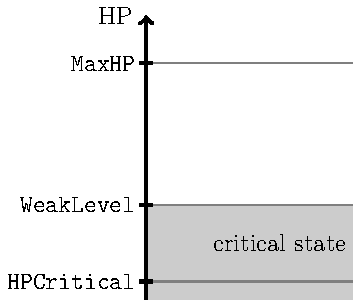
\includegraphics[width=0.3\linewidth]{002_simulation_structure/images/health_global.pdf}
    \caption{The health of the agents is represented by a HP value between \lstinline$HPCritical$ and \lstinline$MaxHP$. All HP values which are below \lstinline$WeakLevel$ are classed as critical. The diagram is not drawn to scale.}
    \label{fig:health_system}
\end{figure}

\subsection{Food and Health: \texorpdfstring{\lstinline$updateHP$}{updateHP}}\label{updateHP}
To increase their HP, agents need to eat. However, the amount an agent's HP improves can saturate in a single day; eating more than a certain amount will provide an agent with no extra benefit to their HP. Moreover, eating more food will lead to diminishing returns in terms of HP change. Mathematically, the ideas of diminishing returns and saturation are well captured by the step response of a 1st-order system \eqref{updateHP_general}:

\begin{equation}\label{updateHP_general}
   \text{newHP}= \text{currentHP} +\underbrace{w(1-e^{\frac{-\text{foodTaken}}{\tau}})}_{\text{HPChange}}
\end{equation}

The two parameters $w$ and $\tau$ are defined at the beginning of the simulation. The shape of this curve is given in \Cref{fig:updateHP} together with some important parameters.

\begin{figure}[htb]%
    \centering
    \subfloat[\centering Overview]{{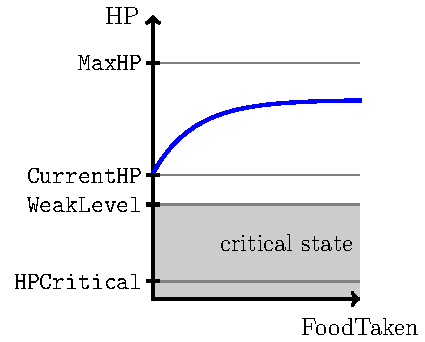
\includegraphics[width=0.36\linewidth]{002_simulation_structure/images/health_updateHP_overview.pdf}}}%
    \qquad
    \subfloat[\centering Detailed representation]{{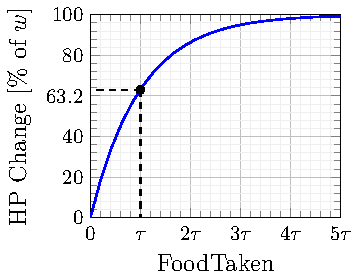
\includegraphics[width=0.36\linewidth]{002_simulation_structure/images/health_updateHP_detailed.pdf}}}%
    \caption{\texttt{updateHP} as a function of the amount of food eaten (``FoodTaken'').}%
    \label{fig:updateHP}%
\end{figure}

It is not possible to gain more HP than $w$ over the duration of one day; this is an intentional limit to prevent an agent's health from improving too quickly. As an example, we can think of an agent that starts from the weak level and wants to reach the maximum HP value. It would take several days for this agent to ``recover'' from this weak level and stabilise its health to a high HP value. 

Note that it is possible for an agent to achieve an HP value that is larger than \texttt{MaxHP} inside \lstinline$hpDecay()$. At the end of each day, the \lstinline$hpDecay()$ function will apply the cost of living and then bound the final HP value by \lstinline$MaxHP$.


Agents in the critical state are treated differently. For these agents, HP is updated according to equation \eqref{updateHP_critical}:

\begin{equation}\label{updateHP_critical}
    \text{newHP} = \min\left\{\text{HPCritical}+\text{HPReqCToW}, \text{currentHP} +w(1-e^{\frac{-\text{foodTaken}}{\tau}})\right\}
\end{equation}

\subsection{Cost of Living: \texorpdfstring{\lstinline$hpDecay()$}{hpDecay}}\label{hpDecay}
At the end of each day, the HP value of the agents will be reduced by the cost of living. The cost of living is larger for an agent with larger HP value than for an agent with lower HP value. This fact is motivated by a simple observation: humans that have stronger bodies and immune systems also need more food to sustain their level of health. The exact relation between HP value, cost of living, and HP value after applying the cost of living is given by the linear relation \eqref{hpDecay_equation}:

\begin{equation}\label{hpDecay_equation}
    \text{newHP} = \text{currentHP}-\left[b + s(\text{currentHP}-\text{WeakLevel})\right]
\end{equation}


The parameter $b$ is a (constant) base cost, and $s$ is the slope of the linear function. These parameters are initialised at the beginning of the simulation. \ToDo{Add a diagram for this?}

To ensure that the HP value at the end of the day is bounded by \texttt{MaxHP}, we slightly modify (\ref{hpDecay_equation}) to produce (\ref{hpDecay_bounded}):

\begin{equation}\label{hpDecay_bounded}
    \text{newHP} =\max\left\{\text{MaxHP}, \text{currentHP}-\left[b + s(\text{currentHP}-\text{WeakLevel})\right]\right\}
\end{equation}

For agents in the critical state that gain \texttt{HPReqCToW} HP in a single day, i.e. their HP after eating is

\begin{equation}\label{HPReqCToW}
    \text{currentHP} \geq \text{HPCritical}+\text{HPReqCToW},
\end{equation}

their HP will be set to \texttt{WeakLevel}:

\begin{equation}\label{hpDecay_critical_upgrade}
    \text{newHP} = \text{WeakLevel}
\end{equation}

Agents in the critical state which do not manage to improve their HP by \lstinline$HPReqCToW$ will be kept in the critical state:

\begin{equation}\label{hpDecay_critical_stay}
    \text{newHP} = \text{HPCritical}
\end{equation}

with the \texttt{daysAtCritical} counter incremented by 1. If \texttt{daysAtCritical} reaches \texttt{MaxDayCritical}, the agent dies and is replaced. This counter is reset to 0 if an agent exits the critical state.